\documentclass[journal]{IEEEtran}
\usepackage{times}
\usepackage{bm,bbm}
\usepackage{amsmath,amssymb}
\usepackage{graphicx,subfigure}
\usepackage{url}
\usepackage{units}
\usepackage{cite,balance}
\usepackage{comment}
\usepackage{multirow}
\usepackage{booktabs}
\usepackage{microtype}
\usepackage{siunitx}
\usepackage{color}

\usepackage[normalem]{ulem} %%%% para tachar texto

\newtheorem{definition}{Definition}
\newtheorem{proposition}{Proposition}
\newcommand{\at}[2][]{#1|_{#2}}

\begin{document}
	
	%\title{SAR image classification using non parametric estimators of Shannon entropy}
	\title{Estimators of the Entropy for SAR Image Classification}
	\author{ Julia~Cassetti, Daiana Delgadino, and Alejandro~C.~Frery,~\IEEEmembership{Senior Member}
		
		%\thanks{This work was supported by Secretar\'ia de Pol\'iticas Universitarias (SPU), CNPq, and Fapeal.}
		
		\thanks{Julia Cassetti and Daiana Delgadino \texttt{julia.cassetti@gmail.com} are with the  Instituto de Desarrollo Humano, Universidad Nacional de General Sarmiento, Pcia. de Buenos Aires, Argentina.}
		
		\thanks{Alejandro C.\ Frery \texttt{alejandro.frery@vuw.ac.nz} is with the School of Mathematics and Statistics, Victoria University of Wellington, New Zealand} 
	}
	
	\maketitle
	
	\begin{abstract}
		
		Remotely sensed data are successfully used for information extraction. 
		In particular SAR imagery, which suffer the presence of speckle noise, needs special models and techniques. 
		In this sense, the $\mathcal G^0$ family of distributions is a suitable model for SAR intensity because it can characterize areas with different degrees of texture. 
		Information theory has gained a place in signal and image processing for parameter estimation and feature extraction.
		Among its tools, the entropy stands out as one of the most expressive features.
		In this paper, we evaluate the performance of several parametric and non parametric Shannon entropy estimators as input for supervised and unsupervised classification algorithms for SAR images.
		These estimators were analyzed through Kappa, overall reliability and accuracy indexes. 
		Finally we apply these estimators to actual data.
		
	\end{abstract}
	
	\begin{keywords}
		Feature extraction, synthetic aperture radar, Shannon entropy, classification.
	\end{keywords}
	
	\IEEEpeerreviewmaketitle
	
	\section{Introduction}
	\label{intro}
	\PARstart{i}{mages} that come from coherent illumination systems, such as those acquired by synthetic aperture radar (SAR) are contaminated by speckle noise. 
	This kind of noise corrupts the image making it difficult to analyze and interpret. 
	
	Under this perspective, statistical procedures are important tools for processing SAR data. 
	The choice of a suitable model and appropriate measures to describe this sort of images is a fundamental point to obtain features that promote a good analysis.
	
	In this sense, the family of distributions $\mathcal{G}^0$~\cite{Frery97} has been extensively used to model SAR data because of its ability to a wide variety of roughness targets. 
	
	Several approaches have been developed in order to obtain expressive and tractable features. 
	In particular, entropy measures have been widely used for this purpose. 
	Estimation parameter~\cite{gambini2015}, classification~\cite{Carvalho2019}, methodologies for constructing
	confidence interval and contrast measures~\cite{Frery2012,Nascimento2009}, and edge detection~\cite{Nascimento2014} are some examples of its application.
	
	Sundry authors have tackled the segmentation and classification SAR images problem using information theory measures. 
	Nobre et al.~\cite{Nobre2016} used Rényi's entropy for monopolarized SAR image segmentation.
	Ferreira et al.~\cite{Ferreira2020} derived a closed-form expression for the Shannon entropy based on the $\mathcal{G}^0$ law for intensity data, and proposed a new entropy-based segmentation method. 
	Carvalho et al.~\cite{Carvalho2019} employed stochastic distances to approach unsupervised classification methodology applied to Polarimetric Synthetic Aperture Radar (PolSAR) images.
	
	The Shannon entropy has been applied to analyzed SAR imagery in several approaches, from inference~\cite{Frery2012} to classification~\cite{Ferreira2020}. 
	Therefore, its estimation deserves attention. 
	Vasicek~\cite{Vasicek76} replaced the distribution function $F$ by the empirical distribution function $F_n$ and used a difference operator in place of the differential operator in the Shannon's entropy expression. 
	Van Es~\cite{VanEs92} studied an entropy estimator based on differences between order statistics. 
	Correa~\cite{Correa95} proposed a new entropy estimator based on local linear regression.
	Al-Omari~\cite{AlOmari2016} and Noughabi and Noughabi~\cite{Noughabi13} presented modified versions of the Ebrahimi et al.~\cite{Ebrahimi94} estimator.
	
	In this paper, we address the classification problem through supervised and unsupervised strategies whose input is the local estimate of the entropy. 
	To this aim, we will evaluate estimators of the entropy, both parametric and non-parametric. 
	In the parametric case we used the relationship between the $\mathcal{G}^0$ and Fisher distributions to obtain an expression of the entropy. 
	In the non parametric case, we will evaluate these estimators in terms of bias, mean square error, computational time and accuracy when classifying a monopolarimetric SAR image. 
	
	\section{The $\mathcal{G}^0$ Model}
	\label{sec_SAR}
	
	The multiplicative model defines the return $Z$ in a monopolarized SAR image as the product of two independent random variables: one corresponding to the backscatter $X$, and the other to the speckle noise $Y$.
	In this manner $Z=X Y$ represents the return $Z$ in each pixel under.
	
	The $\mathcal{G}^{0}$ family of distributions is attractive because of its flexibility to model adequately areas with all types of roughness~\cite{MejailJacoboFreryBustos:IJRS,mejailfreryjacobobustos2001}. 
	For intensity SAR data, this family arises from considering the speckle noise $Y$ modeled as a $\Gamma$ distributed random variable with unitary mean and shape parameter $L\geq1$, the number of looks, while the backscatter $X$ is considered to obey a Reciprocal of Gamma law.  
	The density function for intensity data is given by
	\begin{equation}
		f(z) =\frac{L^{L}\Gamma ( L-\alpha
			) }{\gamma ^{\alpha }\Gamma ( -\alpha ) \Gamma (
			L) }\cdot  
		\frac{z^{L-1}}{( \gamma +zL) ^{L-\alpha }},%
		\label{}
	\end{equation}
	where $-\alpha,\gamma ,z>0$ and $L\geq 1$. 
	The $r$-order moments are
	\begin{equation}
		\text{E}(Z^r) =\Big(\frac{\gamma}{L}\Big)^r\frac{\Gamma ( -\alpha-r )}{ \Gamma (-\alpha) }
		\frac{\Gamma (L+r )}{\Gamma (L)},
		\label{moments_gI0}
	\end{equation}
	provided $\alpha<-r$, and infinite otherwise.
	
	Mejail et al.~\cite{MejailJacoboFreryBustos:IJRS} proved a relationship between $\mathcal G^0$ distributions and the Fisher-Snedekor $F$ law:
	the cumulative distribution function $F_{\alpha,\gamma,L}$ for the return $Z$ is
	\begin{equation}
		F_{\alpha,\gamma,L}(z) = \Upsilon_{2L, -2\alpha}(-\alpha  z / \gamma),
		\label{eq:CDFG0}
	\end{equation}
	for every $z>0$, where $\Upsilon_{2L, -2\alpha}$ is the cumulative distribution function of a Fisher-Snedekor random variable with $2L$ and $-2\alpha$ degrees of freedom.
	This relationship is useful for obtaining an entropy expression. 
	
	\section{Shannon entropy}
	
	%%% ACF Usar la notación usual para entropía: H
	It is well known Shannon's contribution to the creation of what is known Information Theory. 
	Shannon~\cite{Shannon1948} proposed a new way of
	measuring the transmission of information through a channel, thinking of information as a statistical concept. 
	In this regard Shanon's entropy (SE) is defined as
	\begin{align}
		\label{SE}
		H[f(x)]&=-E[\log f(x)]=-\int_{-\infty}^{\infty} f(x) \log f(x) d x\\
		&= \int_{0}^{1} \log \frac{d F^{-1}(x)}{d x} d x,
	\end{align}
	where $X$ is a continuous random variable with probability density function (pdf) $f(x)$ and
	cumulative distribution function (cdf) $F(x)$. 
	
	The entropy of the~$\mathcal{G}^0$ distribution is obtained using~\eqref{eq:CDFG0}.
	Denote $H_{F}$ to entropy under the $F$ model, then the $\mathcal{G}^0$ entropy for intensity data $H_{\mathcal G^0}$ is 
	\begin{align}
		\label{EntropiaFisherGi0}
		H_{\mathcal G^0}(\alpha,\gamma,L)=H_{F}(2 L, - 2 \alpha) -\log\Big(-\dfrac{\alpha}{\gamma}\Big).
	\end{align}
	Using~\eqref{EntropiaFisherGi0}, the
	%%% Por qué "an"? Hay otras? Revisar todo.
	expression of $H_{\mathcal G^0}$ is
	\begin{align}
		\label{EG0}
		H_{\mathcal G^0}(\alpha,\gamma,L)&=-\log \Big(-\frac{\alpha }{\gamma }\Big)-(1-\alpha ) \psi^{(0)}(-\alpha )\\ \nonumber
		&+\log \Big(-\frac{\alpha }{L}\Big)+\frac{1}{2} (2 L-2 \alpha ) \psi ^{(0)}\Big(\frac{1}{2} (2 L-2 \alpha )\Big)\\ \nonumber
		&+\log \big(B(L,-\alpha )\big)+(1-L) \psi^{(0)}(L),
	\end{align}
	where $\psi^{(0)}$ and $B$ are the digamma and beta functions, respectively.
	%%% ACF Sería interesante graficar la entropía para a y g variando, con L fijo
	\begin{figure}[hbt]
		\centering    
		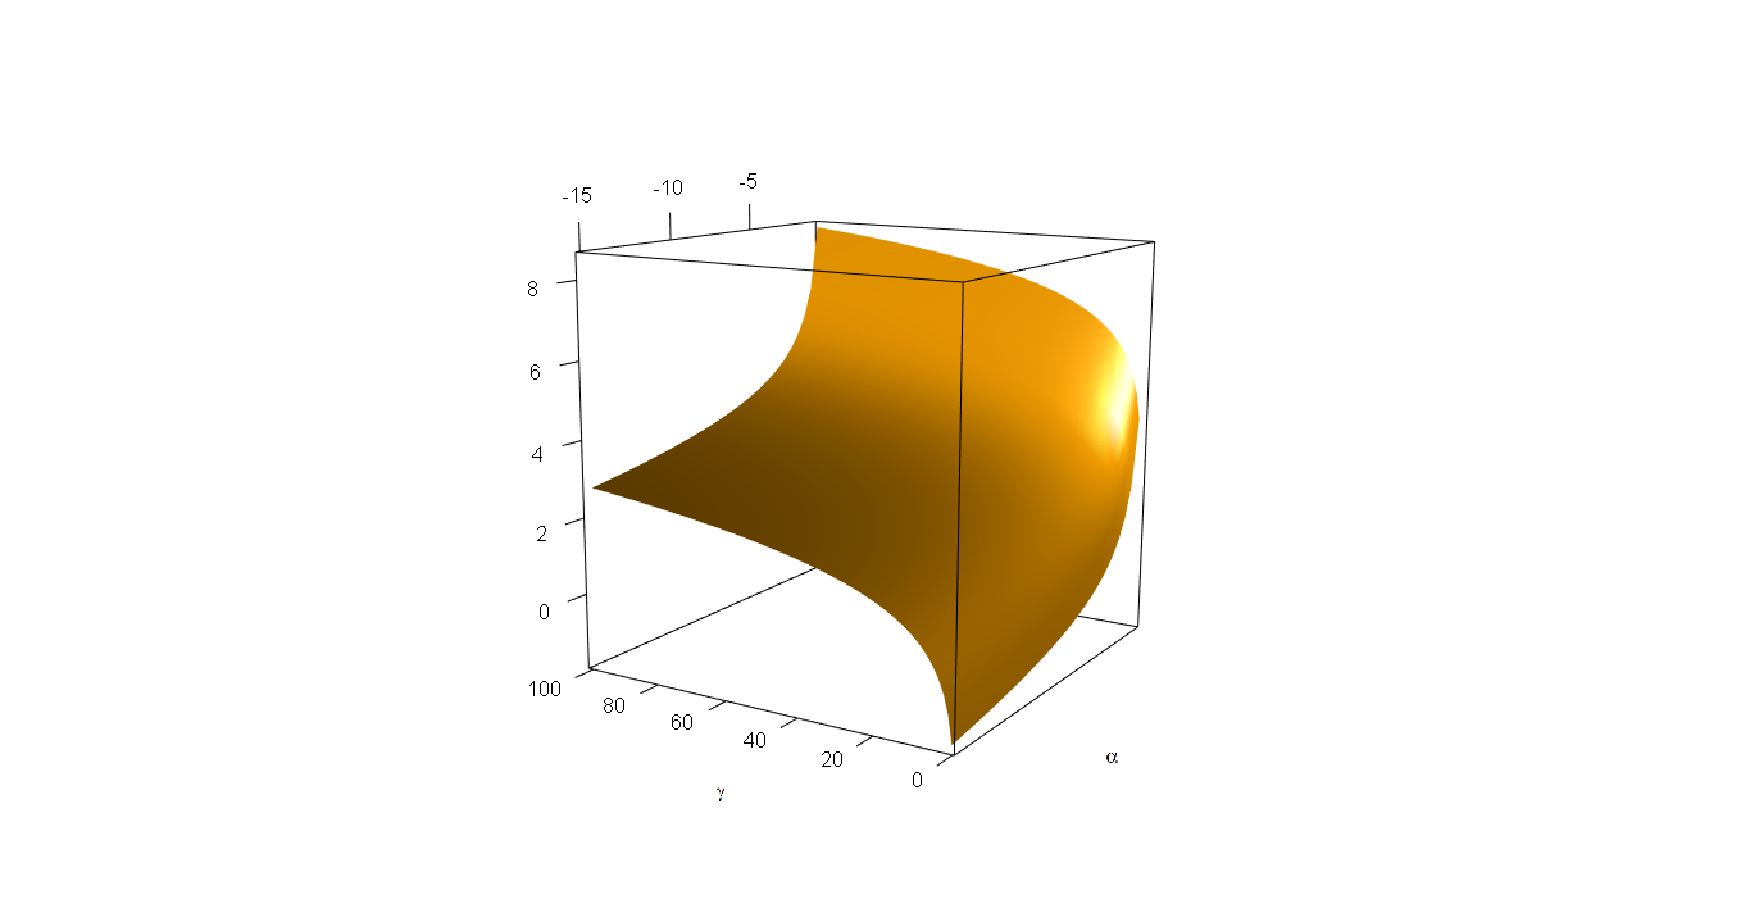
\includegraphics[width=0.6\linewidth]{../../../Figures/CISS2021/HG0L=3_2.pdf}
		\caption{$H_{\mathcal G^0}(\alpha,\gamma,L)$ as a function of alpha and gamma for L=3.\label{figure:HG0}}
	\end{figure}
	
	Figure~\ref{figure:HG0} shows the $H_{\mathcal G^0}(\alpha,\gamma,L)$ theoretical entropy as a function of $\alpha$ and $\gamma$ and $L=3$. It can be shown that, for each fixed  $\gamma$ value, $H_{\mathcal G^0}$ is an injective function. The same behavior happens with $H_{\mathcal G^0}$ when $\alpha$ is a fixed value.
	
	\section{Shannon Entropy Estimators}
	
	Several authors have proposed entropy estimators according to~\eqref{SE}.
	Most of them are based on order statistics of the sample. 
	
	Al-Omari~\cite{AlOmari2016} presented an overview of these estimators and also proposed a new one. 
	From a parametric point of view, is natural to consider the maximum likelihood estimator (MV) of the entropy (HMV).
	
	In this paper we study the following entropy estimators.
	
	\subsection{Maximum likelihood entropy estimator}
	
	
	The optimal asymptotic properties of the MV estimator are well-known. 
	Let $Z_1,\dots, Z_n$ be an independent random sample of size $n$ from the $\mathcal G^0(\alpha,\gamma,L)$ distribution.
	Assume $L$ known.
	A maximum likelihood estimator of $\alpha$ and $\gamma$ for $L$ known, denoted $\widehat\alpha_{\text{ML}}$ and $\widehat\gamma_{\text{ML}}$ respectively, is the value (in the parametric space $\mathbbm R_-\times\mathbbm R_+$), that maximizes the loglikelihood function:
	\begin{align}
		\log \Gamma(L-\widehat\alpha_{\text{ML}})-
		\widehat\alpha_{\text{ML}}\log \widehat\gamma_{\text{ML}} -\log\Gamma(-\widehat\alpha_{\text{ML}}) \nonumber \\
		\mbox{}+\frac{\widehat\alpha_{\text{ML}}-L}{n} \sum_{i=1}^n\log\big(\widehat\gamma_{\text{ML}}+L Z_i\big).
		\label{ML}
	\end{align}
	Its calculation demands numerical maximization routines; we used the L-BFGS-B version of the Broyden-Fletcher-Goldfarb-Shanno (BFGS) method~\cite{Luenberger2008} that allows box constraints.
	This algorithm belongs to the family of quasi-Newton methods. 
	The characteristic of these methods is that they do not require the Hessian matrix, only the gradient.
	
	The ML entropy estimator ($H_{\text{ML}}$)~\cite{CaseBerg01} is, thus,
	\begin{align}
		H_{\text{ML}}=H_{\mathcal G^0}(\widehat{\alpha}_{\text{MV}},\widehat{\gamma}_{\text{MV}},L).
	\end{align}
	
	%; the left-hand-side of~\eqref{rootML} is the gradient of~\eqref{ML}. 
	
	%Function~\eqref{ML} is, in general, unimodal but, depending on the sample, it may be monotonically decreasing. 
	%This behavior is the responsible for the algorithm failing to converge.
	
	
	\subsection{Non parametric entropy estimators}
	\label{nonpar}
	
	We recall the nonparametric entropy estimators studied in~\cite{AlOmari2016}. 
	In all of them we consider that $X_1,\ldots,X_n$ is a random sample from the distribution function $F(x)$, and that $X_{(i)}$ its order statistics, $1\leq i\leq n$. 
	%In the following we present the expression of the studied estimators. 
	%It should be noted that most of the estimators studied in this work 
	%%% ACF m y n van en modo matemático
	%%% ACF citar los artículos originales
	\begin{itemize}
		\item Vasicek~\cite{Vasicek76}:
		\begin{align}
			\label{HV}
			H_{\text{V}(m,n)}=\frac{1}{n} \sum_{i=1}^{n} \log \Big[\frac{n}{2 m}\left(X_{(i+m)}-X_{(i-m)}\right)\Big].
		\end{align}
		%%% ACF Qué es m?
		\item Van Es~\cite{VanEs92}:
		\begin{align}
			\label{HVE}
			H_{\text{VE}(m,n)}&=\frac{1}{n-m} \sum_{i=1}^{n-m}\Big[\frac{n+1}{m}\left(X_{(i+m)}-X_{(i)}\right)\Big] \nonumber\\
			&+\sum_{k=m}^{n} \frac{1}{k}+\log \frac{m}{n+1}.
		\end{align}
		\item Correa~\cite{Correa95}:
		\begin{align}
			\label{HC}
			H_{\text{C}(m,n)}=-\frac{1}{n} \sum_{i=1}^{n} \log \frac{\sum_{j=i-m}^{i+m}(j-i)\left(X_{(j)}-\overline{X}_{(i)}\right)}{n \sum_{j=i-m}^{i+m}\left(X_{(j)}-\overline{X}_{(i)}\right)^{2}},
		\end{align}
		where $\overline{X}_{(i)}=(2 m+1)^{-1} \sum_{j=i-m}^{i+m} X_{(j)}$.
		\item Al-Omari~\cite{AlOmari2014}:
		\begin{align}
			H_{\text{AO}_1(m,n)}=\frac{1}{n} \sum_{i=1}^{n} \log \Big[\frac{n}{\omega_{i} m}\left(X_{(i+m)}-X_{(i-m)}\right)\Big], 
			\label{AHE}
		\end{align}
		where
		\begin{equation*}
			\omega_{i}= \begin{cases}
				1+\frac{1}{2} & \text{ if }1 \leq i \leq m, \\
				2 & \text{ if } m+1 \leq i \leq n-m, \\
				1+\frac{1}{2} & \text{ if } n-m+1 \leq i \leq n,
			\end{cases}
		\end{equation*}
		in which $X_{(i-m)}=X_{(1)}$ for $i \leq m$, and $X_{(i+m)}=X_{(n)}$ for $i \geq n-m$.
		\item Al-Omari alternative proposal~\cite{AlOmari2016}:
		\label{MH}
		\begin{align}
			H_{\text{AO}_2(m,n)}=\frac{1}{n} \sum_{i=1}^{n} \log \Big[\frac{n}{v_{i} m}\left(X_{(i+m)}-X_{(i-m)}\right)\Big],
		\end{align}
		where
		\begin{equation*}
			v_{i}=\begin{cases}
				1+\frac{i-1}{m} & \text{ if }1 \leq i \leq m, \\
				2 & \text{ if } m+1 \leq i \leq n-m, \\
				1+\frac{n-i}{2 m} & \text{ if } n-m+1 \leq i \leq n,
			\end{cases}
		\end{equation*}
		in which $X_{(i-m)}=X_{(1)}$ for $i \leq m$, and $X_{(i+m)}=X_{(n)}$ for $i \geq n-m$.
		\item Ebrahimi~\cite{Ebrahimi94}
		\begin{align}
			H_{\text{E}(m,n)}=\frac{1}{n} \sum_{i=1}^{n} \log \Big[\frac{n}{\tau_{i} m}\left(X_{(i+m)}-X_{(i-m)}\right)\Big],
			\label{HE}
		\end{align}
		where
		\begin{equation*}
			\tau_{i}=\begin{cases}
				1+\frac{i-1}{m} & \text{ if }1 \leq i \leq m, \\
				2 & \text{ if } m+1 \leq i \leq n-m, \\
				1+\frac{n-i}{m} & \text{ if } n-m+1 \leq i \leq n.
			\end{cases}
		\end{equation*}
	\end{itemize}
	
	\section{Simulation study}\label{simulation}
	
	Since most of the estimators depend on the spacing $m$, we first conducted a Monte Carlo study  to choose the value that yields smallest bias and mean squared error (MSE). %We also evaluate the performance of these estimator by accounting for the number of anomalous entropy estimates.
	
	For this study we generated $500$ samples from a $\mathcal{G}^0$ distribution of size $n \in\left\lbrace 9,25,49,81\right\rbrace $ for each roughness value $\alpha \in\left\lbrace -8,-5-3,-1.5\right\rbrace $, each non parametric estimator presented in Section~\ref{nonpar}, $m \leq {n}/{2}$ and also $H_{\text{ML}}$. 
	The sample sizes represent different scenarios of window sizes. 
	
	We then assessed these estimators in the frame of supervised classification by applying SVM, and of unsupervised classification using k-means. 
	We generated simulated images for several values of $\alpha$ and $\gamma$, and used sliding windows of different sizes to generate the entropy map. 
	The classification was performed using these maps as features. 
	The classification methods are evaluated using Kappa and overall accuracy. 
	The parameter estimation methods were tested in an actual SAR image. 
	
	The details and results will be presented in the final paper.
	
	
	
	
	
	
	\section{Computational information}
	\label{conclusion}
	
	
	
	All studies were made in the \texttt R platform and language for statistical computing~\cite{RLanguage} (version~4.0.4).
	
	
	\bibliographystyle{IEEEbib}
	\bibliography{../../../Bibliography/bib_julia2}
	
	
\end{document}